\caulc
\begin{ex}%[1D2N3-4]%[TDMZZ24]%[Bồ Văn Hậu]
	Cho cấp số nhân $\left(u_n\right)$ có $u_1=3$ và có công bội $q=2$. Giá trị của $u_4$ bằng
	\choice
	{$48$}
	{$12$}
	{\True $24$}
	{$6$}
	\loigiai{
		Ta có $u_4=u_1 \cdot q^3=3 \cdot 2^3=24$.
	}
\end{ex}

\begin{ex}%[1D7N2-1]%[TDMZZ24]%[Bồ Văn Hậu]
	Biểu thức đạo hàm của hàm số $y=2^{2x-1}$ là
	\choice
	{\True $y'=2^{2x}\ln 2$}
	{$y'=2^{2x-1}\ln 2$}
	{$y'=2^{2x-2}\ln 2$}
	{$y'=2^{2x-1}$}
	\loigiai{
		Ta có $y'=(2x-1)'\cdot 2^{2x-1} \cdot \ln 2=2 \cdot 2^{2x-1} \cdot \ln 2=2^{2x}\ln 2$.
	}
\end{ex}

\begin{ex}%[1D6H4-5]%[TDMZZ24]%[Bồ Văn Hậu]
	Số nghiệm nguyên của bất phương trình $\log\left(x^2-4x\right)<\log \,(2x)$ là
	\choice
	{$3$}
	{$2$}
	{$4$}
	{\True $1$}
	\loigiai{
		Điều kiện xác định $\heva{&x^2-4x>0\\&2x>0} \Leftrightarrow \heva{&\hoac{&x<0\\&x>4}\\&x>0} \Leftrightarrow x>4$.\\
		Khi đó
		\allowdisplaybreaks
		\begin{eqnarray*}
			&&\log\left(x^2-4x\right)<\log \,(2x)\\
			&\Leftrightarrow&x^2-4x<2x\\
			&\Leftrightarrow&x^2-6x<0\\
			&\Leftrightarrow&0<x<6.
		\end{eqnarray*}
		Kết hợp với điều kiện $x>4$, ta được nghiệm của bất phương trình trên là $4<x<6$.\\
		Vì $x \in \mathbb{Z}$ nên $x=5$.\\
		Vậy bất phương trình đã cho có đúng $1$ nghiệm nguyên.
	}
\end{ex}

\begin{ex}%[2D1N2-1]%[TDMZZ24]%[Bồ Văn Hậu]
	Hàm số $y=x^4-4x^2$ có tất cả bao nhiêu điểm cực tiểu?
	\choice
	{$1$}
	{\True $2$}
	{$3$}
	{$4$}
	\loigiai{
		Tập xác định $\mathscr{D}=\mathbb{R}$.\\
		Ta có $y'=4x^3-8x$. Cho $y'=0 \Leftrightarrow 4x\left(x^2-2\right)=0 \Leftrightarrow \hoac{&x=0\\&x=-\sqrt{2}\\&x=\sqrt{2}.}$\\
		Bảng biến thiên
		\begin{center}
			
\begin{tikzpicture}[>=stealth,line join=round,line cap=round,font=\footnotesize,scale=1]
				\tkzTabInit[nocadre=false,lgt=1,espcl=2,deltacl=0.6]
				{$x$/0.6,$y'$/0.6,$y$/1.5}
				{$-\infty$,$-\sqrt{2}$,$0$,$\sqrt{2}$,$+\infty$}
				\tkzTabLine{,-,0,+,0,-,0,+,}
				\tkzTabVar{+/$+\infty$,-/$-4$,+/$0$,-/$-4$,+/$+\infty$}
			\end{tikzpicture}
		\end{center}
		Dựa vào bảng biến thiên, suy ra hàm số đã cho có $2$ điểm cực tiểu.
	}
\end{ex}

\begin{ex}%[2H2H2-4]%[TDMZZ24]%[Bồ Văn Hậu]
	Trong không gian $Oxyz$, cho điểm $A(3;1;5)$. Khoảng cách từ điểm $A$ đến trục $Ox$ là
	\choice
	{$\sqrt{35}$}
	{$\sqrt{10}$}
	{\True $\sqrt{26}$}
	{$3$ }
	\loigiai{
		Gọi $H$ là hình chiếu vuông góc của điểm $A$ lên trục $Ox$.\\
		Suy ra $H(3;0;0)$ và $AH=\sqrt{(3-3)^2+(0-1)^2+(0-5)^2}=\sqrt{0+1+25}=\sqrt{26}$.\\
		Khoảng cách từ điểm $A$ đến trục $Ox$ chính là độ dài đoạn thẳng $AH=\sqrt{26}$.
	}
\end{ex}

\begin{ex}%[2D1H1-1]%[TDMZZ24]%[Bồ Văn Hậu]
	Hàm số $y=\dfrac{x^2-4x+4}{x-1}$
	\choice
	{đồng biến trên từng khoảng xác định}
	{\True đồng biến trên từng khoảng $(-\infty;0)$; $(2;+\infty)$}
	{nghịch biến trên từng khoảng $(-\infty;0)$; $(2;+\infty)$}
	{nghịch biến trên từng khoảng $(0;1)\cup(1;2)$}
	\loigiai{
		Tập xác định $\mathscr{D}=\mathbb{R}\setminus\{1\}$.\\
		Ta có đạo hàm $y'=\dfrac{x^2-2x}{(x-1)^2}$.\\
		Cho $y'=0 \Rightarrow x^2-2x=0 \Leftrightarrow \hoac{&x=0\\&x=2.}$\\
		Bảng biến thiên
		\begin{center}
			
\begin{tikzpicture}[>=stealth,line join=round,line cap=round,font=\footnotesize,scale=1]
				\tkzTabInit[nocadre=false,lgt=1,espcl=2,deltacl=0.6]
				{$x$/0.6,$y'$/0.6,$y$/2}
				{$-\infty$,$0$,$1$,$2$,$+\infty$}
				\tkzTabLine{,+,0,-,d,-,0,+,}
				\tkzTabVar{-/$-\infty$,+/$-4$,-D+/$-\infty$/$+\infty$,-/$0$,+/$+\infty$}
			\end{tikzpicture}
		\end{center}
		Vậy hàm số đã cho đồng biến trên từng khoảng $(-\infty;0)$ và $(2;+\infty)$.
	}
\end{ex}

\begin{ex}%[2H2H1-3]%[TDMZZ24]%[Bồ Văn Hậu]
	Trong không gian cho hình lập phương $ABCD. A'B'C'D'$. Khẳng định nào sau đây là đúng?
	\choice
	{\True $\left(\overrightarrow{AC},\overrightarrow{DA'}\right)=120^\circ$}
	{$\left(\overrightarrow{AC},\overrightarrow{C'A'}\right)=90^\circ$}
	{$\left(\overrightarrow{AC},\overrightarrow{B'D'}\right)=0^\circ$}
	{$\left(\overrightarrow{AC},\overrightarrow{CB}\right)=45^\circ$}
	\loigiai{
		Hình vẽ
		\begin{center}
			\begin{tikzpicture}[scale=0.7, font=\footnotesize, line join=round, line cap=round, >=stealth,
				declare function={bc=3.5; ba=2; gocB=35;}]
				\path
				(0,0) coordinate (B)
				(gocB:ba) coordinate (A)
				(bc,0) coordinate (C)
				($(C)-(B)+(A)$) coordinate (D)
				($(A)+(90:bc)$) coordinate (A')
				($(B)-(A)+(A')$) coordinate (B')
				($(C)-(A)+(A')$) coordinate (C')
				($(D)-(A)+(A')$) coordinate (D');
				\draw
				(B')--(B)--(C)--(D)--(D')--(A')--(B')--(C')--(D')
				(C)--(C');
				\draw[dashed]
				(A')--(A)--(D)
				(A)--(B);
				\foreach \diem/\goc in {
					A/160, B/-135, C/-45, D/20,
					A'/135, B'/180, C'/-30, D'/45
				}
				\fill (\diem) circle (1.2pt) ++(\goc:0.35) node{$\diem$};
			\end{tikzpicture}
		\end{center}
		Vì $ABCD. A'B'C'D'$ là hình lập phương nên ta có
		\begin{itemize}
			\item $\left(\overrightarrow{AC},\overrightarrow{C'A'}\right)=\left(\overrightarrow{AC},\overrightarrow{CA}\right)=180^\circ$ (vì hai vectơ đối nhau).
			\item $\left(\overrightarrow{AC},\overrightarrow{B'D'}\right)=\left(\overrightarrow{AC},\overrightarrow{BD}\right)=90^\circ$ (vì $\overrightarrow{AC} \perp \overrightarrow{BD}$).
			\item $\left(\overrightarrow{AC},\overrightarrow{CB}\right)=\left(-\overrightarrow{CA},\overrightarrow{CB}\right)=180^\circ-\left(\overrightarrow{CA},\overrightarrow{CB}\right)=180^\circ-45^\circ=135^\circ$.
			\item $\left(\overrightarrow{AC},\overrightarrow{DA'}\right)=\left(\overrightarrow{AC},\overrightarrow{CB'}\right)=\left(-\overrightarrow{CA},\overrightarrow{CB'}\right)=180^\circ-\left(\overrightarrow{CA},\overrightarrow{CB'}\right)=180^\circ-60^\circ=120^\circ$.
		\end{itemize}
	}
\end{ex}

\begin{ex}%[1D5H1-3]%[TDMZZ24]%[Bồ Văn Hậu]
	Cho hai mẫu số liệu ghép nhóm $M_1$, $M_2$ với bảng tần số ghép nhóm như sau\\
	\begin{center}
		Nhóm $M_1$
		\begin{tabular}{|c|c|c|c|c|c|c|}
			\hline
			Nhóm & $[2;3)$ & $[3;4)$ & $[4;5)$ & $[5;6)$ & $[6;7)$ & $[7;8)$ \\
			\hline
			Tần số & $5$ & $5$ & $6$ & $4$ & $6$ & $7$ \\
			\hline
		\end{tabular}
	\end{center}
	\begin{center}
		Nhóm $M_2$
		\begin{tabular}{|c|c|c|c|c|c|c|}
			\hline
			Nhóm & $[4;6)$ & $[6;8)$ & $[8;10)$ & $[10;12)$ & $[12;14)$ & $[14;16)$ \\
			\hline
			Tần số & $5$ & $5$ & $6$ & $4$ & $6$ & $7$ \\
			\hline
		\end{tabular}
	\end{center}
	Hãy so sánh số trung bình cộng $\overline{x}_1$, $\overline{x}_2$ của hai mẫu số liệu $M_1$, $M_2$?
	\choice
	{$\overline{x}_1=\overline{x}_2$}
	{$\overline{x}_1=2\overline{x}_2$}
	{$\overline{x}_1>\overline{x}_2$}
	{\True $\overline{x}_2=2\overline{x}_1$}
	\loigiai{
		Với nhóm $M_1$, ta có
		\begin{center}
			\begin{tabular}{|c|c|c|c|c|c|c|}
				\hline
				Nhóm & $[2;3)$ & $[3;4)$ & $[4;5)$ & $[5;6)$ & $[6;7)$ & $[7;8)$ \\
				\hline
				Giá trị đại diện &$2{,}5$ & $3{,}5$ & $4{,}5$ & $5{,}5$ & $6{,}5$ & $7{,}5$
				\\
				\hline
				Tần số & $5$ & $5$ & $6$ & $4$ & $6$ & $7$ \\
				\hline
			\end{tabular}
		\end{center}
		Giá trị trung bình $\overline{x}_1=\dfrac{5\cdot 2{,}5+5\cdot 3{,}5+6\cdot 4{,}5+4\cdot 5{,}5+6\cdot 6{,}5+7\cdot 7{,}5}{5+5+6+4+6+7}=\dfrac{31}{6}$.\\
		Với nhóm $M_2$, ta có
		\begin{center}
			\begin{tabular}{|c|c|c|c|c|c|c|}
				\hline
				Nhóm & $[4;6)$ & $[6;8)$ & $[8;10)$ & $[10;12)$ & $[12;14)$ & $[14;16)$ \\
				\hline
				Giá trị đại diện & $5$ & $7$ & $9$ & $11$ & $13$ & $15$\\
				\hline
				Tần số & $5$ & $5$ & $6$ & $4$ & $6$ & $7$ \\
				\hline
			\end{tabular}
		\end{center}
		Giá trị trung bình $\overline{x}_2=\dfrac{5\cdot 5+5\cdot 7+6\cdot 9+4\cdot 11+6\cdot 13+7\cdot 15}{5+5+6+4+6+7}=\dfrac{31}{3}$.\\
		Ta thấy $\overline{x}_2=2\overline{x}_1$.
	}
\end{ex}

\begin{ex}%[2D4H2-1]%[TDMZZ24]%[Bồ Văn Hậu]
	Cho biết nguyên hàm của hàm số $y=f(x)$ trên $\mathbb{R}$ là $F(x)$ và có $F(0)=2F(1)=4$. Giá trị của tích phân $\displaystyle\int\limits_{0}^{1} f(x)\mathrm{\,d}x$ tương ứng bằng
	\choice
	{\True $-2$}
	{$2$}
	{$0$}
	{$6$}
	\loigiai{
		Ta có $F(0)=2F(1)=4 \Rightarrow \heva{&F(0)=4\\&F(1)=2.}$\\
		Mặt khác
		\[\displaystyle\int\limits_{0}^{1} f(x)\mathrm{\,d}x=F(1)-F(0)=2-4=-2.\]
	}
\end{ex}

\begin{ex}%[1H8H7-3]%[TDMZZ24]%[Bồ Văn Hậu]
	Cho hình chóp tứ giác đều $S. ABCD$ có tất cả các cạnh bằng $a$. Thể tích của khối chóp $S. ABC$ tương ứng bằng
	\choice
	{$\dfrac{a^3\sqrt{2}}{6}$}
	{$\dfrac{a^3\sqrt{2}}{4}$}
	{$\dfrac{a^3}{3}$}
	{\True $\dfrac{a^3\sqrt{2}}{12}$}
	\loigiai{
		\immini{Gọi $O$ là tâm của hình vuông $ABCD$.\\ Vì $S. ABCD$ là hình chóp tứ giác đều nên $SO \perp (ABCD)$.\\
			Ta có $S_{\Delta ABC}=\dfrac{1}{2}S_{ABCD}=\dfrac{a^2}{2}$.\\
			Xét tam giác $SAO$ vuông tại $O$, ta có
			\[SO=\sqrt{SA^2-AO^2}=\sqrt{a^2- \left(\dfrac{a\sqrt{2}}{2}\right)^2}=\dfrac{a\sqrt{2}}{2}.\]
			Thể tích khối chóp $S. ABC$ là
			\[V_{S. ABC}=\dfrac{1}{3}S_{ABC} \cdot SO=\dfrac{1}{3} \cdot \dfrac{a^2}{2} \cdot \dfrac{a\sqrt{2}}{2}=\dfrac{a^3\sqrt{2}}{12}.\]}{\begin{tikzpicture}[scale=0.8, font=\footnotesize, line join=round, line cap=round, >=stealth, declare function={bc=4; ba=2; h=4; gocB=30;}]
				\path
				(0,0) coordinate (B)
				(gocB:ba) coordinate (A)
				(bc,0) coordinate (C)
				($(C)-(B)+(A)$) coordinate (D)
				($(A)!0.5!(C)$) coordinate (O)
				($(O)+(90:h)$) coordinate (S);
				\draw (B)--(C)--(D)--(S)--cycle (S)--(C);
				\draw[dashed] (C)--(A)--(D)--(B) (O)--(S)--(A)--(B);
				\foreach \diem/\goc in {A/160, B/-135, C/-45, D/20, S/90, O/-90}
				\fill[black] (\diem) circle (1.2pt) ++(\goc:0.35) node{$\diem$};
		\end{tikzpicture}}
	}
\end{ex}

\begin{ex}%[2H5H3-3]%[TDMZZ24]%[Bồ Văn Hậu]
	Trong không gian $Oxyz$, mặt cầu $(S)$ có tâm $I(2;1;-4)$ và tiếp xúc với mặt phẳng $(P)\colon 2x+y-2z-1=0$. Phương trình mặt cầu $(S)$ là
	\choice
	{\True $(S)\colon (x-2)^2+(y-1)^2+(z+4)^2=4^2$}
	{$(S)\colon (x-2)^2+(y-1)^2+(z+4)^2=4$}
	{$(S)\colon (x+2)^2+(y+1)^2+(z-4)^2=4^2$}
	{$(S)\colon (x+2)^2+(y+1)^2+(z-4)^2=4$}
	\loigiai{
		Mặt cầu $(S)$ tiếp xúc với mặt phẳng $(P)$ nên $(S)$ có bán kính là
		\[R=\mathrm{d}\big(I,(P)\big)= \dfrac{\left|2\cdot 2+1-2\cdot(-4)-1\right|}{\sqrt{2^2+1^2+(-2)^2}}=\dfrac{12}{3}=4.\]
		Phương trình mặt cầu $(S)$ tâm $I(2;1;-4)$ và bán kính $R=4$ là
		\[(x-2)^2+(y-1)^2+(z+4)^2=4^2.\]
	}
\end{ex}

\begin{ex}%[2D4H3-3]%[TDMZZ24]%[Bồ Văn Hậu]
	Cho hình phẳng $(H)$ giới hạn bởi $f(x)=x^2-6x$, trục hoành $Ox$. Khi cho hình phẳng $(H)$ quay quanh trục $Ox$ thì thể tích khối tròn xoay thu được là
	\choice
	{$36\pi$}
	{$\dfrac{2\,218\pi}{3}$}
	{$84\pi$}
	{\True $\dfrac{1\,296\pi}{5}$}
	\loigiai{
		Phương trình hoành độ giao điểm của đồ thị hàm số $f(x)=x^2-6x$ và trục hoành $Ox$ ($y=0$) là
		\[x^2-6x=0 \Leftrightarrow \hoac{&x=0\\&x=6.}\]
		Thể tích khối tròn xoay thu được khi quay hình phẳng $(H)$ quanh trục $Ox$ là
		\allowdisplaybreaks
		\begin{eqnarray*}
			V &=& \pi \displaystyle\int\limits_{0}^{6} \left(x^2-6x\right)^2 \mathrm{\,d}x\\
			&=& \pi \displaystyle\int\limits_{0}^{6} \left(x^4-12x^3+36x^2\right) \mathrm{\,d}x\\
			&=& \pi \left(\dfrac{x^5}{5}-3x^4+12x^3\right)\bigg|_0^6 \\
			&=& \pi \left(\dfrac{6^5}{5}-3\cdot 6^4+12\cdot 6^3-0\right)\\
			&=& \dfrac{1\,296\pi}{5}.
		\end{eqnarray*}
	}
\end{ex}
\cauds
\begin{ex}%[2D1H2-1]%[Dương Công Tạo]
	Trong mặt phẳng $Oxy$, cho hàm số $y = f (x) = x^6 -6x^4$ có đồ thị $(C)$.
	\choiceTF
	{\True $f'(x) = 6x^5 - 24x^3$}
	{\True Hàm số $f(x)$ đồng biến trên các khoảng $(-2;0)$ và $(2;+\infty)$}
	{\True $(C)$ có ba điểm cực trị tạo tạo thành tam giác cân}
	{$(C)$ có ba điểm cực trị tạo thành tam giác có diện tích bằng $128$}
	\loigiai{
		\begin{itemchoice}
			\itemch Xét hàm số $y = f (x) = x^6 -6x^4$ trên khoảng $(-\infty;+\infty)$.\\
			Ta có hàm số $f'(x) = 6x^5 -24x^3=6x^3\left(x^2-4\right)$.
			\itemch Ta có $f'(x)=0\Leftrightarrow 6x^3\left(x^2-4\right)=0\Leftrightarrow\hoac{&x=0\\&x=\pm 2.}$\\
			Bảng biến thiên
			\begin{center}
				
\begin{tikzpicture}[>=stealth]
					\tkzTabInit[nocadre=false,lgt=1.5,espcl=2,deltacl=0.6]{$x$/.7 ,$f'(x)$/.7,$f(x)$/2}
					{$-\infty$ , $-2$ , $0$ , $2$ , $+\infty$}
					\tkzTabLine{ , + , 0 , - , 0 , - , 0,+}
					\tkzTabVar{+/$+\infty$ , -/$-32$ , +/$0$ , -/$-32$ , +/$+\infty$}
				\end{tikzpicture}
			\end{center}
			Dựa vào bảng biến thiên, ta thấy hàm số $f(x)$ đồng biến trên các khoảng $(-2;0)$ và $(2;+\infty)$.
			\itemch Gọi $O(0;0)$, $A(-2;-32)$ và $B(2;-32)$ là ba điểm cực trị của đồ thị $(C)$ của hàm số.\\
			Ta có $OA=OB=\sqrt{(2-0)^2+(-32-0)^2}=2\sqrt{257}$; $AB=4$. \\
			Suy ra $\triangle OAB$ cân tại $O$ hay $(C)$ có ba điểm cực trị tạo tạo thành tam giác cân.
			\itemch Gọi $H(0;-32)$ là trung điểm của $AB$ thì $OH\perp AB$.\\
			Ta có $S_{OAB}=\dfrac{1}{2}\cdot OH\cdot AB=\dfrac{1}{2}\cdot 32\cdot 4=64$.
		\end{itemchoice}
	}
\end{ex}

\begin{ex}%[TDMZZ24]%[Hà Văn Hảo]%[2D4V2-6]
	Sau buổi học, An chở Bình về trên xe máy điện. Xe đang chạy với tốc độ $10$ m/s thì phát hiện đèn tín hiệu giao thông chuyển đỏ cách vị trí xe $120$ m. Ba giây sau đó, xe máy bắt đầu giảm tốc với vận tốc được cho bởi $v_1(t) = at + b$ m/s ($a, b \in \mathbb{R}$, $a < 0$), trong đó $t$ là thời gian (tính bằng giây) kể từ khi xe bắt đầu giảm tốc. Khi xe máy đến vị trí đèn tín hiệu, đèn vẫn còn đỏ và xe dừng hẳn. Sau khi đèn chuyển xanh, xe tiếp tục di chuyển với vận tốc được cho bởi $v_2(t) = mt^2 + nt$ m/s ($m, n \in \mathbb{R}$, $m < 0$), trong đó $t$ là thời gian (tính bằng giây) kể từ lúc đèn bắt đầu chuyển xanh, hai bạn dừng lại ở một cửa hàng bên đường. Biết rằng thời gian xe máy đi từ vị trí đèn tín hiệu xanh đến cửa hàng là $36$ giây và vận tốc lớn nhất của xe trên đoạn đường này là $15$ m/s.
	\choiceTF
	{\True Quãng đường xe máy đi được từ lúc bắt đầu giảm tốc lần thứ nhất đến khi dừng hẳn tại vị trí đèn tín hiệu là $90$ m}
	{\True Giá trị của hệ số $b$ là $10$}
	{\True Xe máy dừng hẳn tại vị trí đèn tín hiệu sau $18$ giây kể từ khi bắt đầu giảm tốc lần thứ nhất}
	{Khoảng cách từ vị trí đèn tín hiệu đến vị trí cửa hàng là $480$ m}
	\loigiai{
		\begin{itemchoice}
			\itemch Trong $3$ giây đầu kể từ khi thấy đèn đỏ, xe chuyển động thẳng đều với vận tốc $v = 10$ m/s. Quãng đường đi được là $s_0 = 10 \cdot 3 = 30$ m.\\
			Khoảng cách từ vị trí bắt đầu giảm tốc đến đèn tín hiệu là $s_1 = 120 - 30 = 90$ m.
			\itemch Tại thời điểm bắt đầu giảm tốc ($t = 0$), vận tốc của xe là $v_1(0) = 10$ m/s.\\
			Thay vào công thức $v_1(t) = at + b$, ta có $a \cdot 0 + b = 10 \Rightarrow b = 10$.
			\itemch Gọi $t_1$ là thời gian từ lúc bắt đầu giảm tốc đến khi dừng hẳn ($v_1(t_1) = 0$).\\
			Ta có $at_1 + 10 = 0 \Rightarrow a = -\dfrac{10}{t_1}$.\\
			Quãng đường giảm tốc là
			\[s_1 = \displaystyle\int\limits_0^{t_1} (at + 10)\,\mathrm{d}t = \left. \left( \dfrac{at^2}{2} + 10t \right) \right|_0^{t_1} = \dfrac{at_1^2}{2} + 10t_1 = 90.\]
			Thay $a = -\dfrac{10}{t_1}$ vào $\dfrac{-10}{2t_1} \cdot t_1^2 + 10t_1 = 90 \Leftrightarrow -5t_1 + 10t_1 = 90 \Leftrightarrow 5t_1 = 90 \Leftrightarrow t_1 = 18$ giây.
			\itemch Xét giai đoạn từ đèn xanh đến cửa hàng, hàm vận tốc $v_2(t) = mt^2 + nt$ với $t \in [0; 36]$.\\
			Xe dừng lại tại cửa hàng sau $36$ giây nên
			\[v_2(36) = 0 \Rightarrow m(36)^2 + n(36) = 0 \Rightarrow n = -36m.\]
			Khi đó $v_2(t) = mt^2 - 36mt$. \\
			Vận tốc đạt cực đại tại $t = -\dfrac{-36m}{2m} = 18$ giây.\\
			Vận tốc cực đại $v_2(18) = m(18)^2 - 36m(18) = -324m = 15 \Rightarrow m = -\dfrac{15}{324} = -\dfrac{5}{108}$.\\
			Suy ra $n = -36 \cdot \left( -\dfrac{5}{108} \right) = \dfrac{5}{3}$.\\
			Quãng đường từ đèn đến cửa hàng là
			\[s_2 = \displaystyle\int\limits_0^{36} \left( -\dfrac{5}{108}t^2 + \dfrac{5}{3}t \right)\,\mathrm{d}t = \left. \left( -\dfrac{5}{324}t^3 + \dfrac{5}{6}t^2 \right) \right|_0^{36} = 360 \, \text{m}.\]
		\end{itemchoice}
	}
\end{ex}

\begin{ex}%[2D6V2-4]%[TDMZZ24]%[Vũ Hồng Toàn]
	Tiến hành gieo ngẫu nhiên một con súc sắc cân đối đồng chất hai lần liên tiếp. Gọi $A$ là biến cố lần thứ nhất xuất hiện số chấm lớn hơn $2$, $B$ là biến cố tổng số chấm ở hai lần gieo nhỏ hơn $6$.
	\choiceTF
	{\True $\mathrm{P}(A)=\dfrac{2}{3}$}
	{\True $\mathrm{P}(B\mid A)=\dfrac{1}{8}$}
	{\True $\mathrm{P}(B)=\dfrac{5}{18}$}
	{\True $\mathrm{P}(A\mid B)=\dfrac{3}{10}$}
	\loigiai{
		Không gian mẫu của phép thử gieo một con súc sắc hai lần liên tiếp có số phần tử là \[n(\Omega) = 6 \cdot 6 = 36.\]
		Các kết quả thuận lợi cho $B$ là các cặp $(x; y)$ sao cho $x + y < 6$, bao gồm
		\[\left\{(1;1), (1;2), (1;3), (1;4), (2;1), (2;2), (2;3), (3;1), (3;2), (4;1)\right\}\]
		\begin{itemchoice}
			\itemch Các kết quả thuận lợi cho $A$ là các cặp $(x; y)$ với $x \in \{3; 4; 5; 6\}$ và $y \in \{1; 2; 3; 4; 5; 6\}$.\\
			Do đó, số phần tử của biến cố $A$ là $n(A) = 4 \cdot 6 = 24$.\\
			Xác suất của biến cố $A$ là $\mathrm{P}(A) = \dfrac{24}{36} = \dfrac{2}{3}$.
			\itemch Các kết quả thuận lợi cho $A \cap B$ là $\{(3;1), (3;2), (4;1)\}$.\\
			Do đó, số phần tử của biến cố $A \cap B$ là $n(A \cap B) = 3$.\\
			Xác suất của biến cố $A \cap B$ là $\mathrm{P}(A \cap B) = \dfrac{3}{36} = \dfrac{1}{12}$.
			\itemch Số phần tử của biến cố $B$ là $n(B) = 10$.\\
			Xác suất của biến cố $B$ là $\mathrm{P}(B) = \dfrac{10}{36} = \dfrac{5}{18}$.
			\itemch Ta có
			\[\mathrm{P}(A\mid B) = \dfrac{\mathrm{P}(A \cap B)}{\mathrm{P}(B)} = \dfrac{\dfrac{1}{12}}{\dfrac{5}{18}} = \dfrac{3}{10}.\]
		\end{itemchoice}
	}
\end{ex}

\begin{ex}%[2H5V3-4]%[TDMZZ24]%[Văn Minh Thoại]
	Gắn hệ trục tọa độ $Oxyz$ (đơn vị trên mỗi trục là mét), một nguồn sáng đặt ở vị trí $S(4;3;2)$ có bán kính chiếu sáng là $70$ m. Một chiếc drone $X$ đang bay thẳng đều từ vị trí $A(-60;110;14)$ đến vị trí $B(70;-30;14)$ với vận tốc không đổi $12$ m/s. Trên drone $X$ có một nguồn sáng với bán kính chiếu sáng là $25$ m.
	\choiceTF
	{Vị trí $A$ nhận được ánh sáng của nguồn sáng $S$}
	{\True Phương trình tham số đường bay của drone $X$ là $\heva{&x=-60+13t\\&y=110-14t\\&z=14}$, $t\in\mathbb{R}$}
	{Trong quá trình drone $X$ bay, có thời điểm nguồn sáng $S$ nằm trong vùng chiếu sáng của drone $X$}
	{Drone $X$ bay trong vùng chiếu sáng của $S$ trong khoảng thời gian là $7$ giây \textit{(tính theo đơn vị giây và làm tròn kết quả đến hàng đơn vị)}}
	\loigiai{
		Ta có vectơ chỉ phương của đường thẳng $AB$ là $\overrightarrow{AB}=(130;-140; 0)=10(13;-14; 0)$.\\
		Chọn vectơ $\overrightarrow{u}=(13;-14; 0)$ làm vectơ chỉ phương cho quỹ đạo bay của drone.\\
		Đường bay của drone là đường thẳng $\Delta$ đi qua $A$ và $B$.
		\begin{itemchoice}
			\itemch Khoảng cách từ nguồn sáng $S$ đến vị trí $A$ ban đầu là
			\[SA=\sqrt{(-60-4)^2+(110-3)^2+(14-2)^2}=\sqrt{(-64)^2+107^2+12^2}=\sqrt{15\,689}\approx 125{,}25 \;\text{(m)}\]
			Vì $SA\approx 125{,}25$ m$>R_S=70$ m, nên ánh sáng từ $S$ không thể chiếu tới vị trí $A$.
			\itemch Đường bay $\Delta$ của drone đi qua $A(-60; 110; 14)$ và nhận $\overrightarrow{u}=(13;-14; 0)$ làm vectơ chỉ phương có phương trình tham số là $\heva{&x=-60+13t\\&y=110-14t\\&z=14}$ với $t\in\mathbb{R}$.
			\itemch
			\begin{center}
				\begin{tikzpicture}[>=stealth,declare function={Rs=3.5; Rx=1.25; d=1.43; halfL=sqrt (Rs*Rs-d*d);},line join=round,line cap=round,,scale=1]
					
					\path
					(0,0) coordinate (H)
					(90:d) coordinate (S)
					(180:halfL) coordinate (M)
					(0:halfL) coordinate (N)
					(180:5.5) coordinate (A)
					(0:5.5) coordinate (B);
					\draw[->] (N) -- (B) node[pos=0.5,sloped,above,font=\scriptsize] {$\Delta$};
					\draw (A)--(M);
					\path pic[draw,angle radius=6pt]{right angle=S--H--N};
					\draw[dashed] (S) -- (H) node[pos=0.5,sloped,above,font=\scriptsize] {$d$};
					\draw (S) circle (Rs);
					\begin{scope}[shift={(S)}]
						\draw[dashed] plot[domain=0:180] ({Rs*cos (\x)},{0.25*Rs*sin (\x)});
						\draw plot[domain=180:360] ({Rs*cos (\x)},{0.25*Rs*sin (\x)});
					\end{scope}
					\draw[dashed] (H) circle (Rx);
					\begin{scope}[shift={(H)}]
						\draw[dashed] plot[domain=0:180] ({Rx*cos (\x)},{0.25*Rx*sin (\x)});
						\draw[dashed] plot[domain=180:360] ({Rx*cos (\x)},{0.25*Rx*sin (\x)});
					\end{scope}
					\draw[dashed] (S) -- (M) node[pos=0.5,sloped,above,font=\scriptsize] {$R_S$};
					\path (H) + (-60:Rx) coordinate (Rx_edge);
					\draw[->,dashed] (H) -- (Rx_edge) node[pos=0.6,sloped,below,font=\scriptsize] {$R_X$};
					\draw[line width=1.2pt,dashed] (M) -- (N);
					\path
					($(M)+(270:2.5)$) coordinate (Dm)
					($(N)+(270:2.4)$) coordinate (Dn);
					\draw[dashed] (M) -- ($(M)+(270:2.6)$);
					\draw[dashed] (N) -- ($(N)+(270:2.6)$);
					\draw[<->] (Dm) -- (Dn) node[pos=0.5,fill=white,font=\scriptsize] {$L$};
					\foreach \p/\pos in {S/90,A/90,B/90}{
						\draw[fill,ball color=red] (\p) circle (1pt) node[shift={(\pos:9pt)},font=\scriptsize] {$\p$};}
					\node[shift={(-135:10mm)},font=\scriptsize] at (H) {$X$};					
				\end{tikzpicture}
			\end{center}
			Ta có $\overrightarrow{AS}=(64;-107;-12)$ và $\overrightarrow{u}=(13;-14; 0)$.\\
			Khi đó \[\left[\overrightarrow{AS},\overrightarrow{u}\right]=\left(\begin{vmatrix}-107&-12\\-14& 0
			\end{vmatrix};\begin{vmatrix}-12& 64\\0& 13
			\end{vmatrix};\begin{vmatrix}64&-107\\13&-14
			\end{vmatrix}\right)=(-168;-156; 495).\]
			Khoảng cách ngắn nhất từ $S$ đến đường bay $\Delta$ của drone là \[\mathrm{d}\big(S,\Delta\big)=\dfrac{\left|\left[\overrightarrow{AS},\overrightarrow{u}\right]\right|}{\left|\overrightarrow{u}\right|}=\dfrac{\sqrt{(-168)^2+(-156)^2+495^2}}{\sqrt{13^2+(-14)^2+0^2}}=\dfrac{\sqrt{297585}}{\sqrt{365}}\approx 28{,}55\;\text{(m)}.\]
			Vì khoảng cách ngắn nhất từ $S$ đến quỹ đạo bay là $\mathrm{d}\approx 28{,}55$ m$>R_X=25$ m, nên nguồn sáng $S$ không bao giờ nằm trong vùng chiếu sáng của drone.
			\itemch Drone $X$ bay trong vùng chiếu sáng của $S$ tương ứng với đoạn thẳng (dây cung) bị cắt bởi mặt cầu tâm $S$, bán kính $R_S=70$ và đường thẳng $\Delta$.\\
			Độ dài quãng đường drone bay trong vùng sáng là
			\[L = 2\sqrt{R_S^2 - \mathrm{d}^2\big(S, \Delta\big)} = 2\sqrt{70^2 - \dfrac{297\,585}{365}} = 2\sqrt{4\,900 - \dfrac{59\,517}{73}} = 2\sqrt{\dfrac{298\,183}{73}} \approx 127{,}82 \;\text{(m)}.\]
			Thời gian drone bay qua vùng chiếu sáng là
			\[T = \dfrac{L}{v} = \dfrac{127{,}82}{12} \approx 11\ne7\;\text{(giây)}.\]
		\end{itemchoice}
	}
\end{ex}
\caukq
\begin{ex}%[1H8H7-9]%[TDMZZ24]%[Lê Hồ Quang Minh]
	Một khối đá có dạng hình lăng trụ tam giác đều $ABC. A'B'C'$ với cạnh đáy bằng $30\text{ cm}$, khoảng cách từ điểm $A$ đến mặt phẳng $(A'BC)$ bằng $18\text{ cm}$. Hãy tính theo đơn vị đêximét khối thể tích khối đá đã cho \textit{(không làm tròn ở các phép tính trung gian và làm tròn kết quả cuối cùng đến hàng phần mười)}?
	\par\shortans[oly]{9,7}
	\loigiai{
		\immini{
			Vì $ABC. A'B'C'$ là hình lăng trụ tam giác đều nên đáy $ABC$ là tam giác đều cạnh $a = 30\text{ cm}$ và các cạnh bên $AA', BB', CC'$ vuông góc với mặt đáy.\\
			Gọi $H$ là trung điểm của $BC$.\\
			Do $\Delta ABC$ đều nên $AH \perp BC$.\\
			Mặt khác, do lăng trụ đứng nên $AA' \perp (ABC) \Rightarrow AA' \perp BC$.\\
			Suy ra $BC \perp (A'AH) \Rightarrow (A'BC) \perp (A'AH)$ theo giao tuyến $A'H$.\\
			Trong mặt phẳng $(A'AH)$, kẻ $AK \perp A'H$ tại $K$.\\
			Khi đó $AK \perp (A'BC) \Rightarrow \mathrm{d}\left(A, (A'BC)\right) = AK = 18\text{ cm}$.
		}{
			\begin{tikzpicture}[scale=0.7, font=\footnotesize, line join=round, line cap=round, >=stealth]
				\coordinate (A) at (0,0);
				\coordinate (B) at (-1.5,-1.8);
				\coordinate (C) at (4,-1.8);
				\coordinate (H) at ($(B)!0.5!(C)$);
				\path (A) +(0,5.5) coordinate (A');
				\coordinate (B') at ($(B)+(A')-(A)$);
				\coordinate (C') at ($(C)+(A')-(A)$);
				\path[name path=lineAHe] (A')--(H);
				\coordinate (S) at ($(A)!1.5!90:(H)$);
				\path[name path=lineAK] (A)--($(A)!(A')!(H)$);
				\coordinate (K) at ($(A')!(A)!(H)$);
				\draw (A')--(B')--(C')--cycle (B)--(C)--(C')--(B')--cycle;
				\draw[dashed] (C)--(A')--(B)--(A)--(C) (A')--(A)--(H)--cycle (A)--(K);
				\pic[draw, angle eccentricity=1.5, angle radius=2mm]{right angle=A--K--A'};
				\pic[draw, angle eccentricity=1.5, angle radius=1.8mm]{right angle=A--H--C};
				\foreach \i/\g in {A/160, B/-135, C/-45, A'/90, B'/135, C'/45, H/-90, K/0}
				\fill[black] (\i) circle (1pt) +(\g:2.5mm) node {$\i$};
			\end{tikzpicture}
		}
		\noindent Xét tam giác $ABC$ đều cạnh $30\text{ cm}$, đường cao $AH$ là
		\[AH = 30 \cdot \dfrac{\sqrt{3}}{2} = 15\sqrt{3}\text{ cm}.\]
		Diện tích đáy của khối lăng trụ đều là
		\[S_{ABC} = \dfrac{30^2\sqrt{3}}{4} = 225\sqrt{3}\text{ cm}^2.\]
		Xét tam giác $A'AH$ vuông tại $A$ với đường cao $AK$, áp dụng hệ thức lượng ta có:
		\allowdisplaybreaks
		\begin{eqnarray*}
			\dfrac{1}{AK^2} = \dfrac{1}{AA'^2} + \dfrac{1}{AH^2} &\Leftrightarrow& \dfrac{1}{18^2} = \dfrac{1}{AA'^2} + \dfrac{1}{\left(15\sqrt{3}\right)^2} \\
			&\Leftrightarrow& \dfrac{1}{AA'^2} = \dfrac{13}{8\,100} \\
			&\Rightarrow& AA' = \dfrac{90\sqrt{13}}{13}\text{ cm}.
		\end{eqnarray*}
		Thể tích khối lăng trụ tam giác đều theo đơn vị centimet khối ($\text{cm}^3$) là:
		\[V = S_{ABC} \cdot AA' = 225\sqrt{3} \cdot \dfrac{90\sqrt{13}}{13} = \dfrac{20\,250\sqrt{39}}{13} \text{ cm}^3 \approx 9{,}7 \text{ dm}^3.\]
	}
\end{ex}
\begin{ex}%[Dự án]%[Tên file]%[2H5V2-8]
	Từ mặt đất tại hai điểm có hai vật cùng xuất phát theo hai hướng lên trên. Để xác định cho chúng có thể gặp nhau trên không trung để va chạm vào nhau người ta gắn hệ trục toạ độ $Oxyz$ vào với một điểm trùng với gốc toạ độ $O$ và chuyển động với vectơ vận tốc $\overrightarrow{v}_1 = (3;1;4)$ và vật thứ hai là điểm $A$ có toạ độ $A(10;50;30)$ và chuyển động với vectơ vận tốc $\overrightarrow{v}_2 = (a;b;2)$. Hãy tính $(4a+b)$?
	\shortans[]{7}
	\loigiai{
		Giả sử hai vật gặp nhau tại điểm $B$ trên không trung sau khoảng thời gian $t$ ($t>0$).
		Vị trí của vật thứ nhất sau thời gian $t$ là điểm $B$, ta có $\overrightarrow{OB} = \overrightarrow{v}_1 \cdot t = (3t; t; 4t)$, suy ra $B(3t; t; 4t)$.
		Vị trí của vật thứ hai sau thời gian $t$ cũng là điểm $B$, ta có $\overrightarrow{AB} = \overrightarrow{v}_2 \cdot t = (at; bt; 2t)$, suy ra tọa độ của $B$ được tính theo $A$ là
		\[ \heva{&x_B = 10 + at \\ &y_B = 50 + bt \\ &z_B = 30 + 2t.} \]
		Vì hai vật gặp nhau tại $B$ tại cùng một thời điểm $t$ nên tọa độ điểm $B$ ở hai cách biểu diễn phải giống nhau. Ta có hệ phương trình:
		\[ \heva{&3t = 10 + at \\ &t = 50 + bt \\ &4t = 30 + 2t} \Leftrightarrow \heva{&3t = 10 + at \quad (1) \\ &t = 50 + bt \quad (2) \\ &2t = 30 \Rightarrow t = 15.} \]
		Thay $t=15$ vào phương trình $(1)$ và $(2)$, ta được:
		\begin{eqnarray*}
			\heva{&3 \cdot 15 = 10 + 15a \\ &15 = 50 + 15b} &\Leftrightarrow& \heva{&15a = 35 \\ &15b = -35} \\
			&\Leftrightarrow& \heva{&a = \dfrac{7}{3} \\ &b = -\dfrac{7}{3}.}
		\end{eqnarray*}
		Khi đó, giá trị biểu thức cần tính là
		\[ 4a + b = 4 \cdot \dfrac{7}{3} + \left(-\dfrac{7}{3}\right) = \dfrac{28}{3} - \dfrac{7}{3} = \dfrac{21}{3} = 7. \]
		Vậy $(4a+b)=7$.
	}
\end{ex}
\begin{ex}%[2D4C3-1]%[TDMZZ24-19-TLN]%[Đỗ Đường Hiếu]
	\immini[thm]{Trên mặt phẳng tọa độ $Oxy$ có đơn vị dài trên mỗi trục là $10$ cm, cho hình tròn $(C)$ có bán kính bằng $20$ cm, $(C)$ tiếp xúc với parabol $(P)\colon y=x^2$ và tiếp xúc với trục hoành như hình vẽ. Hãy tính diện tích phần hình phẳng được tô màu theo đơn vị cm$^2$ (\textit{làm tròn kết quả đến hàng đơn vị}).}
	{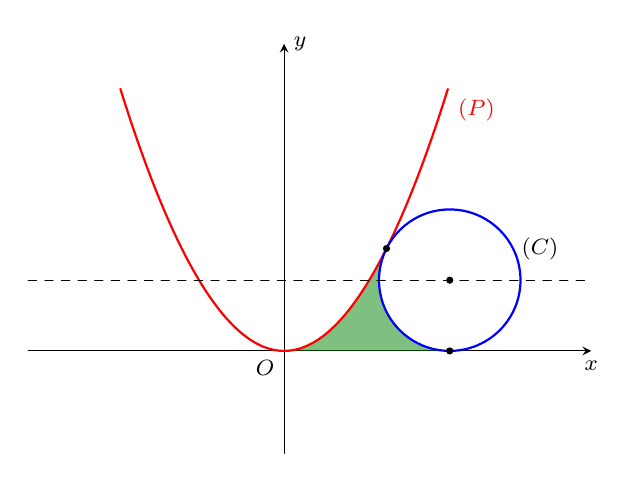
\begin{tikzpicture}[line join = round, line cap = round,>=stealth,font=\footnotesize,scale=1.3]
			\pgfmathsetmacro\a{0.5+0.5*sqrt(5)}
			\pgfmathsetmacro\b{1.25-0.25*sqrt(5)}
			\draw[->] (-2.5,0) -- (3,0) node[below] {$x$};
			\draw[->] (0,-1) -- (0,3) node[right] {$y$};
			\node at (0,0) [below left] {$O$};
			\begin{scope}
				\clip (-2.5,-1) rectangle (3,3);
				\fill[green!50!black, opacity=0.5] (0,0) -- plot[domain=0:1] (\x, {(\x)^2}) -- (1,1)--(\a,0) -- cycle;
				\fill[white] (\a,\b) circle (\b);
				\draw[thick, domain=-1.6:1.6, samples=100, red] plot (\x, {(\x)^2}) node[below right] {$(P)$};
				\draw[blue, thick] (\a,\b) circle (\b);
			\end{scope}
			\draw[dashed] (-2.5,\b) -- (3,\b);
			\fill (\a,\b) circle (1pt);
			\fill (\a,0) circle (1pt);
			\fill (1,1) circle (1pt);
			\node at (2.5,1) {$(C)$};
	\end{tikzpicture}}
	\par\shortans{203}
	\loigiai{
		Đổi đơn vị: $1$ đơn vị trên trục tọa độ tương ứng $1$ cm.\\
		Bán kính hình tròn là $R = 20\text{ cm} = 2$ đơn vị.\\
		Gọi tâm hình tròn là $I\left(a; b\right)$. Vì $(C)$ tiếp xúc với trục hoành nên $b = R = 2$. Suy ra $I\left(a; 2\right)$.\\
		Đường tròn $(C)$ tiếp xúc với $(P)\colon y=x^2$ tại điểm $M(m; m^2)$.\\
		Tại $M$, tiếp tuyến của $(P)$ có hệ số góc $k = 2m$. Tiếp tuyến của $(C)$ vuông góc với $IM$, nên hệ số góc $IM$ là $k_{IM}=-\dfrac{1}{2m}$.\\
		Mặt khác, hệ số góc của đường thẳng $IM$ là $k_{IM}=\dfrac{y_M-y_I}{x_M-x_I}=\dfrac{m^2-2}{m-a}$.\\
		Từ đó ta có $-\dfrac{1}{2m}=\dfrac{m^2-2}{m-a}\Rightarrow a=2m^3-3m$.\\
		Mặt khác $IM^2=4\Leftrightarrow (m-a)^2+(m^2-2)^2=4\Leftrightarrow (4m-2m^3)^2+(m^2-2)^2=4$.\\
		Sử dụng máy tính cầm tay ta tìm được $m\approx 1{,}6103\Rightarrow a\approx 3{,}5203$.\\
		Phương trình $(C)\colon (x-a)^2 + (y-2)^2 = 4$.\\
		Phần đường tròn nằm bên trái đường thẳng $x=a$ là $x=a-\sqrt{4y-y^2}$.\\
		Phần parabol $(P)$ nằm bên phải trục tung $Oy$ là $x=\sqrt{y}$.\\
		Diện tích phần tô màu là
		$$S=\displaystyle\int\limits_0^{m^2}\left[\left(a-\sqrt{4y-y^2}\right)-\sqrt{y}\right]\mathrm{\,d}y\approx 2{,}0346.$$
		Diện tích phần tô màu theo đơn vị cm$^2$ bằng $S=2{,}0346\cdot 10^2\approx 203$.
	}
\end{ex}

\begin{ex}%[0D0V2-6]%[TDMZZ24]%[Nguyễn Đức Tuấn Anh]
	\immini[thm]{
		Trên mặt phẳng $Oxy$, cho hình vuông $OABD$ có cạnh bằng $8$. Đường tròn $(C)$ nội tiếp hình vuông $OABD$. Điểm $E$ nằm trên cạnh $AB$ sao cho $EA=3EB$. Chọn ngẫu nhiên một điểm có tọa độ nguyên thuộc hình tròn $(C)$. Hãy tính xác suất để điểm được chọn thuộc hình phẳng được tô màu (\textit{làm tròn kết quả đến hàng phần trăm})?
	}{
		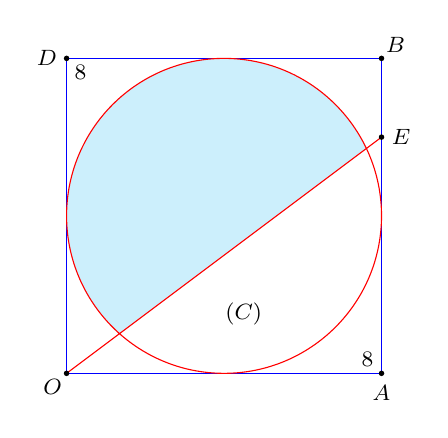
\begin{tikzpicture}[scale=0.5, font=\footnotesize, line join=round, line cap=round, >=stealth]
			\path (0,0) coordinate (O) 
			(8,0) coordinate (A) 
			(8,8) coordinate (B) 
			(0,8) coordinate (D) 
			(8,6) coordinate (E) 
			(4,4) coordinate (I);
			\begin{scope}
				\clip (I) circle (4);
				\fill[cyan!20] (O) -- (E) -- (B) -- (D) -- cycle;
			\end{scope}
			\draw[blue] (O) -- (A) -- (B) -- (D) -- cycle;
			\draw[red] (I) circle (4) (O) -- (E);
			\foreach \p/\ang in {O/-135, A/-90, B/45, D/180, E/0}
			\fill (\p)circle (2pt) node[shift=(\ang:0.25)] {$\p$};
			\path (A) ++(135:0.5) node {$8$}
			(D) ++(-45:0.5) node {$8$}
			(4.5, 1.5) node {$(C)$};
		\end{tikzpicture}
	}
	\par\shortans{0{,}63}
	\loigiai{
		\immini{
			Chọn hệ trục tọa độ $Oxy$ như hình vẽ, ta có $O(0;0)$, $A(8;0)$, $B(8;8)$ và $D(0;8)$.\\
			Đường tròn $(C)$ nội tiếp hình vuông $OABD$ nên có tâm $I(4;4)$ và bán kính $R=4$. \\
			Phương trình của hình tròn $(C)$ là $(x-4)^2 + (y-4)^2 \le 16$.\\
			Điểm $E$ thuộc cạnh $AB$ (có phương trình $x=8$). \\
			Vì $EA = 3EB$ và $AB=8$ nên $y_E - y_A = \dfrac{3}{4}(y_B - y_A) \Rightarrow y_E = 6$.\\
			Suy ra $E(8;6)$.\\
			Đường thẳng $OE$ đi qua gốc tọa độ và $E(8;6)$ nên có phương trình
			\[y = \dfrac{6}{8}x \Leftrightarrow 3x - 4y = 0.\]}{
			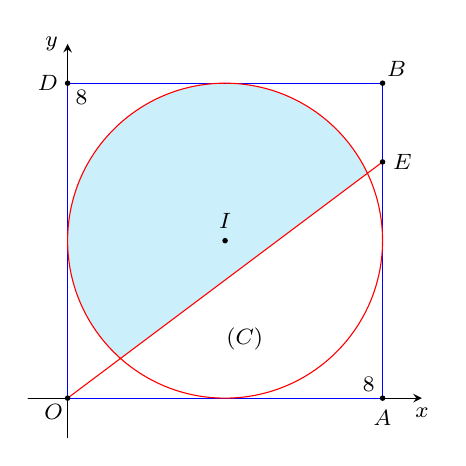
\begin{tikzpicture}[scale=0.5, font=\footnotesize, line join=round, line cap=round, >=stealth]
				\path (0,0) coordinate (O) 
				(8,0) coordinate (A) 
				(8,8) coordinate (B) 
				(0,8) coordinate (D) 
				(8,6) coordinate (E) 
				(4,4) coordinate (I);
				\begin{scope}
					\clip (I) circle (4);
					\fill[cyan!20] (O) -- (E) -- (B) -- (D) -- cycle;
				\end{scope}
				\draw[->] (-1,0)--(9,0)node[below]{$x$};
				\draw[->] (0,-1)--(0,9)node[left]{$y$};
				\draw[blue] (O) -- (A) -- (B) -- (D) -- cycle;
				\draw[red] (I) circle (4) (O) -- (E);
				\foreach \p/\ang in {O/-135,A/-90,B/45,D/180,E/0,I/90}
				\fill (\p)circle (2pt) node[shift=(\ang:0.25)] {$\p$};
				\path (A) ++(135:0.5) node {$8$}
				(D) ++(-45:0.5) node {$8$}
				(4.5, 1.5) node {$(C)$};
			\end{tikzpicture}
		}
		\noindent Tập hợp các điểm có tọa độ nguyên thuộc $(C)$ là các điểm $(x;y)$ thỏa mãn $(x-4)^2 + (y-4)^2 \le 16$ với $x$, $y \in \mathbb{Z}$. \\
		Ta liệt kê số điểm ứng với mỗi hoành độ $x$ như sau
		\begin{itemize}
			\item Với $x=0$ hoặc $x=8$, ta có $(y-4)^2 \le 0 \Rightarrow y=4$ (có $2$ điểm).
			\item Với $x=1$ hoặc $x=7$, ta có $(y-4)^2 \le 7 \Rightarrow y \in \{2;3;4;5;6\}$ (có $10$ điểm).
			\item Với $x=2$ hoặc $x=6$, ta có $(y-4)^2 \le 12 \Rightarrow y \in \{1;2;3;4;5;6;7\}$ (có $14$ điểm).
			\item Với $x=3$ hoặc $x=5$, ta có $(y-4)^2 \le 15 \Rightarrow y \in \{1;2;3;4;5;6;7\}$ (có $14$ điểm).
			\item Với $x=4$, ta có $(y-4)^2 \le 16 \Rightarrow y \in \{0;1;2;3;4;5;6;7;8\}$ (có $9$ điểm).
		\end{itemize}
		Số phần tử của không gian mẫu là $n(\Omega) = 2 + 10 + 14 + 14 + 9 = 49$.\\
		Phần hình phẳng được tô màu là phần của hình tròn $(C)$ nằm phía trên đường thẳng $OE$.\\
		Do đó, các điểm $(x;y)$ thuộc phần tô màu sẽ thỏa mãn điều kiện $y \ge \dfrac{3}{4}x$. \\
		Số điểm thỏa mãn trong từng trường hợp là
		\begin{itemize}
			\item $x=0 \Rightarrow y=4 \ge 0$ (có $1$ điểm).
			\item $x=1 \Rightarrow y \ge 0{,}75 \Rightarrow y \in \{2;3;4;5;6\}$ (có $5$ điểm).
			\item $x=2 \Rightarrow y \ge 1{,}5 \Rightarrow y \in \{2;3;4;5;6;7\}$ (có $6$ điểm).
			\item $x=3 \Rightarrow y \ge 2{,}25 \Rightarrow y \in \{3;4;5;6;7\}$ (có $5$ điểm).
			\item $x=4 \Rightarrow y \ge 3 \Rightarrow y \in \{3;4;5;6;7;8\}$ (có $6$ điểm).
			\item $x=5 \Rightarrow y \ge 3{,}75 \Rightarrow y \in \{4;5;6;7\}$ (có $4$ điểm).
			\item $x=6 \Rightarrow y \ge 4{,}5 \Rightarrow y \in \{5;6;7\}$ (có $3$ điểm).
			\item $x=7 \Rightarrow y \ge 5{,}25 \Rightarrow y \in \{6\}$ (có $1$ điểm).
			\item $x=8 \Rightarrow y=4 \ge 6$, vô lý (có $0$ điểm).
		\end{itemize}
		Gọi $A$ là biến cố \lq\lq Điểm được chọn thuộc hình phẳng được tô màu\rq\rq. \\
		Số kết quả thuận lợi cho biến cố $A$ là $n(A) = 1 + 5 + 6 + 5 + 6 + 4 + 3 + 1 = 31$.\\
		Xác suất của biến cố $A$ là $\mathrm{P}(A) = \dfrac{n(A)}{n(\Omega)} = \dfrac{31}{49} \approx 0{,}63$.
	}
\end{ex}
\begin{environment-name}
	content
\end{environment-name}
\begin{ex}%[0D0C2-3]%[TDM42]%[Nguyễn Văn Sang]
	Có $18$ chiếc bàn học được chia thành $3$ dãy $6$ hàng, mỗi hàng có ba chiếc bàn như hình vẽ. Thầy chủ nhiệm xếp ngẫu nhiên $18$ em học sinh của lớp vào $18$ chiếc bàn này sao cho mỗi em ngồi một bàn. Biết rằng lớp có $4$ học sinh giỏi xuất sắc, $3$ em học sinh giỏi, $2$ em học sinh khá và còn lại là trung bình. Gọi $p$ là xác suất để xếp được mỗi hàng không có nhiều hơn một học sinh cùng xuất sắc hoặc cùng giỏi hoặc cùng khá. Hãy tính $1000p$ \textit{(làm tròn kết quả đến hàng đơn vị)}?
	\begin{center}
		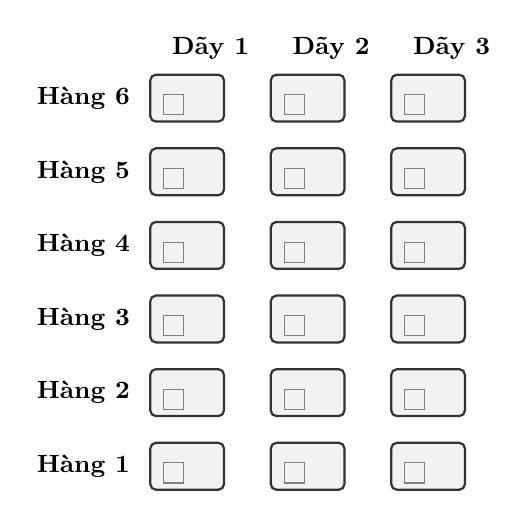
\begin{tikzpicture}[scale=0.85, >=stealth]
			% Đã đổi toàn bộ hình vẽ sang tone Trắng - Đen - Xám chuẩn đề thi in giấy
			\foreach \r in {1,...,6} {
				\foreach \c in {1,...,3} {
					\draw[thick, fill=gray!10, draw=black!80, rounded corners=2pt] (\c*1.8-0.6, \r*1.1-0.4) rectangle ++(1.1,0.7);
					\draw[thin, draw=black!50] (\c*1.8-0.4, \r*1.1-0.3) rectangle ++(0.3,0.3);
				}
				\node[font=\small\bfseries] at (0.2, \r*1.1-0.05) {Hàng \r};
			}
			\node[font=\bfseries\small] at (2.1, 7.3) {Dãy 1};
			\node[font=\bfseries\small] at (3.9, 7.3) {Dãy 2};
			\node[font=\bfseries\small] at (5.7, 7.3) {Dãy 3};
		\end{tikzpicture}
	\end{center}
	\par\shortans[0]{242}
	\loigiai{
		\textbf{Bước 1: Tính số phần tử của không gian mẫu}\\
		Xếp ngẫu nhiên $18$ học sinh vào $18$ chiếc bàn phân biệt
		$$n(\Omega) = 18! \text{ (cách)}$$
		\textbf{Bước 2: Phân tích bài toán và Phương pháp giải}\\
		Lớp có $4$ bạn Xuất sắc (XS), $3$ bạn Giỏi (G), $2$ bạn Khá (K) và $9$ bạn Trung bình (TB).
		Điều kiện bài toán: \textit{Mỗi hàng ngang không có quá $1$ XS, không quá $1$ G, không quá $1$ K}. (Lưu ý: Các nhóm này được phép ngồi chung hàng với nhau, miễn là không trùng loại).\\
		Để tránh sai sót, ta chia quá trình sắp xếp thành 2 công đoạn:
		\begin{itemize}
			\item \textbf{Công đoạn 1:} Thiết kế sơ đồ chỗ ngồi (Lần lượt chọn và "dán nhãn" ghế cho nhóm XS, rồi đến G, rồi đến K).
			\item \textbf{Công đoạn 2:} Mời từng học sinh cụ thể vào đúng chiếc ghế đã dán nhãn.
		\end{itemize}
		\textbf{Bước 3: Thiết kế sơ đồ chỗ ngồi (Công đoạn 1)}\\
		\textbf{1. Chọn ghế cho nhóm Xuất sắc (XS):}
		\begin{itemize}
			\item Chọn $4$ hàng (trong $6$ hàng), mỗi hàng chọn $1$ ghế: Có $\mathrm{C}_6^4 \cdot 3^4 = \mathbf{1215} \text{ (cách)}$.
			\item \textit{Tình trạng lớp lúc này:} Gồm \textbf{$4$ hàng} bị chiếm $1$ chỗ (còn $2$ trống) và \textbf{$2$ hàng} chưa ai ngồi (còn $3$ trống).
		\end{itemize}
		\textbf{2. Chọn ghế cho nhóm Giỏi (G) và Khá (K) bằng Bảng:}
		Nhóm G ($3$ bạn) chọn ghế ở $3$ hàng khác nhau. Ta xét số lượng hàng mà nhóm G "ngồi chung" với nhóm XS, từ đó suy ra chỗ trống còn lại cho nhóm K ($2$ bạn)
		\begin{center}
			\renewcommand{\arraystretch}{1.5}
			\begin{tabular}{|p{0.3\linewidth}|p{0.3\linewidth}|p{0.32\linewidth}|}
				\hline
				\centering\textbf{Trường hợp nhóm G} & \centering\textbf{Số cách cho nhóm G} & \multicolumn{1}{c|}{\textbf{Cấu trúc ghế trống để xếp Khá}} \\ \hline
				
				\textbf{TH1: Ngồi chung XS $1$ hàng} \newline
				\textit{(G chọn $1$ hàng đang có 2 trống \newline \& $2$ hàng đang có 3 trống)}
				& Chọn chung: $\mathrm{C}_4^1 \cdot 2^1 = 8$ \newline
				Chọn riêng: $\mathrm{C}_2^2 \cdot 3^2 = 9$ \newline
				$\Rightarrow 8 \times 9 = \mathbf{72}$ (cách)
				& $\bullet$ \textbf{1 hàng:} còn $1$ trống. \newline
				$\bullet$ \textbf{5 hàng:} còn $2$ trống. \newline
				$\Rightarrow$ Cách xếp 2 K: \textbf{50 cách (*)} \\ \hline
				
				\textbf{TH2: Ngồi chung XS $2$ hàng} \newline
				\textit{(G chọn $2$ hàng đang có 2 trống \newline \& $1$ hàng đang có 3 trống)}
				& Chọn chung: $\mathrm{C}_4^2 \cdot 2^2 = 24$ \newline
				Chọn riêng: $\mathrm{C}_2^1 \cdot 3^1 = 6$ \newline
				$\Rightarrow 24 \times 6 = \mathbf{144}$ (cách)
				& $\bullet$ \textbf{2 hàng:} còn $1$ trống. \newline
				$\bullet$ \textbf{3 hàng:} còn $2$ trống. \newline
				$\bullet$ \textbf{1 hàng:} còn $3$ trống. \newline
				$\Rightarrow$ Cách xếp 2 K: \textbf{49 cách (*)} \\ \hline
				
				\textbf{TH3: Ngồi chung XS $3$ hàng} \newline
				\textit{(G chọn $3$ hàng đang có 2 trống \newline \& $0$ hàng đang có 3 trống)}
				& Chọn chung: $\mathrm{C}_4^3 \cdot 2^3 = 32$ \newline
				Chọn riêng: $1$ \newline
				$\Rightarrow 32 \times 1 = \mathbf{32}$ (cách)
				& $\bullet$ \textbf{3 hàng:} còn $1$ trống. \newline
				$\bullet$ \textbf{1 hàng:} còn $2$ trống. \newline
				$\bullet$ \textbf{2 hàng:} còn $3$ trống. \newline
				$\Rightarrow$ Cách xếp 2 K: \textbf{48 cách (*)} \\ \hline
			\end{tabular}
		\end{center}
		\textit{(*) Tính toán số cách xếp chỗ cho nhóm Khá (chọn $2$ ghế ở $2$ hàng khác nhau):}
		\begin{itemize}
			\item \textbf{TH1:} Cả $2$ ghế vào hàng (2 trống): $\mathrm{C}_5^2 \cdot 2^2 = 40$. Hoặc chia vào hàng (1 trống) và hàng (2 trống): $\mathrm{C}_1^1 \cdot 1 \cdot \mathrm{C}_5^1 \cdot 2 = 10$. Tổng $= \mathbf{50}$.
			\item \textbf{TH2:} Căn cứ vào số lượng hàng trống ở cột 3, ta có $$(\mathrm{C}_2^2 \cdot 1^2) + (\mathrm{C}_3^2 \cdot 2^2) + (\mathrm{C}_2^1 \cdot 1 \cdot \mathrm{C}_3^1 \cdot 2) + (\mathrm{C}_2^1 \cdot 1 \cdot \mathrm{C}_1^1 \cdot 3) + (\mathrm{C}_3^1 \cdot 2 \cdot \mathrm{C}_1^1 \cdot 3) = \mathbf{49}$$
			\item \textbf{TH3:} Căn cứ vào số lượng hàng trống ở cột 3, ta có $$(\mathrm{C}_3^2 \cdot 1^2) + (\mathrm{C}_2^2 \cdot 3^2) + (\mathrm{C}_3^1 \cdot 1 \cdot \mathrm{C}_1^1 \cdot 2) + (\mathrm{C}_3^1 \cdot 1 \cdot \mathrm{C}_2^1 \cdot 3) + (\mathrm{C}_1^1 \cdot 2 \cdot \mathrm{C}_2^1 \cdot 3) = \mathbf{48}$$
		\end{itemize}
		
		Tổng số sơ đồ vị trí hợp lệ cho $3$ nhóm XS, G, K là
		$$m = 1215 \times \Big[ (72 \times 50) + (144 \times 49) + (32 \times 48) \Big] = \mathbf{14.813.280} \text{ (sơ đồ)}.$$
		\textbf{Bước 4: Tính xác suất (Công đoạn 2)}\\
		Ứng với $14.813.280$ sơ đồ đã định sẵn, ta xếp học sinh vào phòng
		\begin{itemize}
			\item Hoán vị các em XS, G, K vào đúng ghế nhóm mình: $4! \cdot 3! \cdot 2!$ (cách).
			\item Hoán vị $9$ em Trung bình vào $9$ ghế trống còn lại: $9!$ (cách).
		\end{itemize}
		Xác suất cần tìm của bài toán là
		$$p = \dfrac{14.813.280 \times 4! \times 3! \times 2! \times 9!}{18!} \approx 0,241805$$
		Ta có $1000p = 241,805$. Làm tròn đến hàng đơn vị, kết quả là $\boxed{242}$.
	}
\end{ex}